\documentclass[12pt, a4paper]{article}

% Базовые пакеты для русского языка
\usepackage[utf8]{inputenc}
\usepackage[T2A]{fontenc}
\usepackage[russian]{babel}

% Математика
\usepackage{amsmath, amsfonts, amssymb}

% Графика
\usepackage{graphicx}
\usepackage{float}

% Настройка полей
\usepackage[left=2cm, right=2cm, top=2cm, bottom=2cm]{geometry}

% Кликабельные ссылки
\usepackage{hyperref}
\hypersetup{
    colorlinks=true,
    linkcolor=blue,
    filecolor=magenta,      
    urlcolor=cyan,
}

\begin{document}

\title{Исследование характеристик СМО с помощью имитационного моделирования}
\author{Лепин Владислав Дмитриевич}
\date{}
\maketitle

\section*{Цели работы}
\begin{enumerate}
    \item Запустить эксперимент для СМО M/M/1 для определения среднего времени нахождения заявки в системе и сравнить с аналитикой.
    \item Провести эксперимент для СМО M/U/1 и сравнить с формулой Поллачека-Хинчина.
    \item Модифицировать код для реализации M/M/c/c (система с отказами) и проанализировать вероятность блокировки и среднее время в системе в зависимости от количества каналов $c$.
\end{enumerate}

\section*{Что было сделано}
В качестве основы использовался предоставленный код для моделирования на C++. В ходе работы:
\begin{itemize}
    \item Исправлены названия переменных для соответствия их физическому смыслу (например, размер очереди заменен на размер всей системы).
    \item Добавлена поддержка трех режимов работы: M/M/1, M/U/1 и M/M/c/c.
    \item Написан скрипт на Python для проведения серий экспериментов. Для ускорения расчетов реализовано параллельное выполнение через \texttt{ThreadPoolExecutor}. Эксперименты выполняются пачками (размер пачки равен числу логических ядер процессора) до достижения необходимой ширины доверительного интервала (параметр \texttt{target\_beta}) или лимита по прогонам.
\end{itemize}

\section*{1. Исследование M/M/1}
Простейшая одноканальная система с пуассоновским входящим потоком и экспоненциальным временем обслуживания. Среднее время пребывания заявки в системе (Sojourn Time) $W$ определяется формулой:
\[ W = \frac{1}{\mu - \lambda} \]
Условие стационарности: $\rho = \lambda/\mu < 1$. При приближении интенсивности поступления $\lambda$ к интенсивности обслуживания $\mu$ время нахождения в системе устремляется в бесконечность.

\begin{figure}[H]
    \centering
    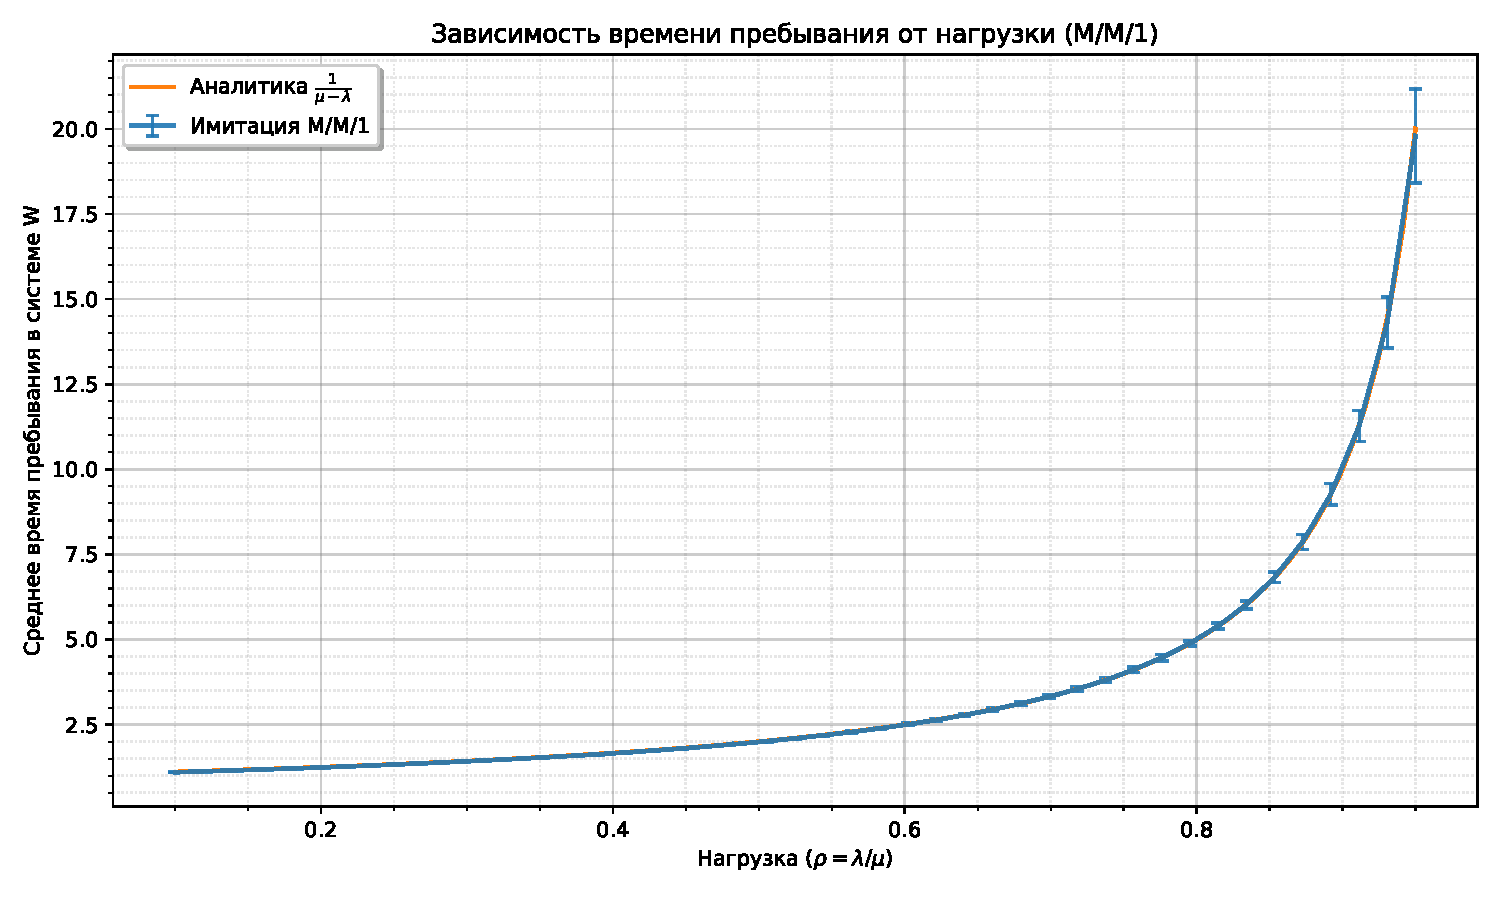
\includegraphics[width=1\textwidth]{mm1.pdf} 
    \caption{Зависимость времени пребывания от нагрузки для системы M/M/1}
\end{figure}

\section*{2. Исследование M/U/1}
Для систем с произвольным распределением времени обслуживания (M/G/1) используется формула Поллачека-Хинчина. Среднее время пребывания $W$ выражается через моменты времени обслуживания $S$:
\[ W = E[S] + \frac{\lambda E[S^2]}{2(1 - \rho)} \]

В нашем случае время обслуживания распределено равномерно $U(0, \frac{2}{\mu})$. Рассчитаем его характеристики:
\begin{itemize}
    \item Математическое ожидание: $E[S] = \frac{0 + \frac{2}{\mu}}{2} = \frac{1}{\mu}$
    \item Дисперсия: $Var[S] = \frac{(\frac{2}{\mu} - 0)^2}{12} = \frac{4}{12\mu^2} = \frac{1}{3\mu^2}$
    \item Второй начальный момент: $E[S^2] = Var[S] + (E[S])^2 = \frac{1}{3\mu^2} + \frac{1}{\mu^2} = \frac{4}{3\mu^2}$
\end{itemize}

Подставляя эти значения в формулу, получаем аналитическое выражение для M/U/1:
\[ W_{M/U/1} = \frac{1}{\mu} + \frac{\lambda \frac{4}{3\mu^2}}{2(1 - \rho)} = \frac{1}{\mu} \left( 1 + \frac{2\rho}{3(1 - \rho)} \right) \]

\begin{figure}[H]
    \centering
    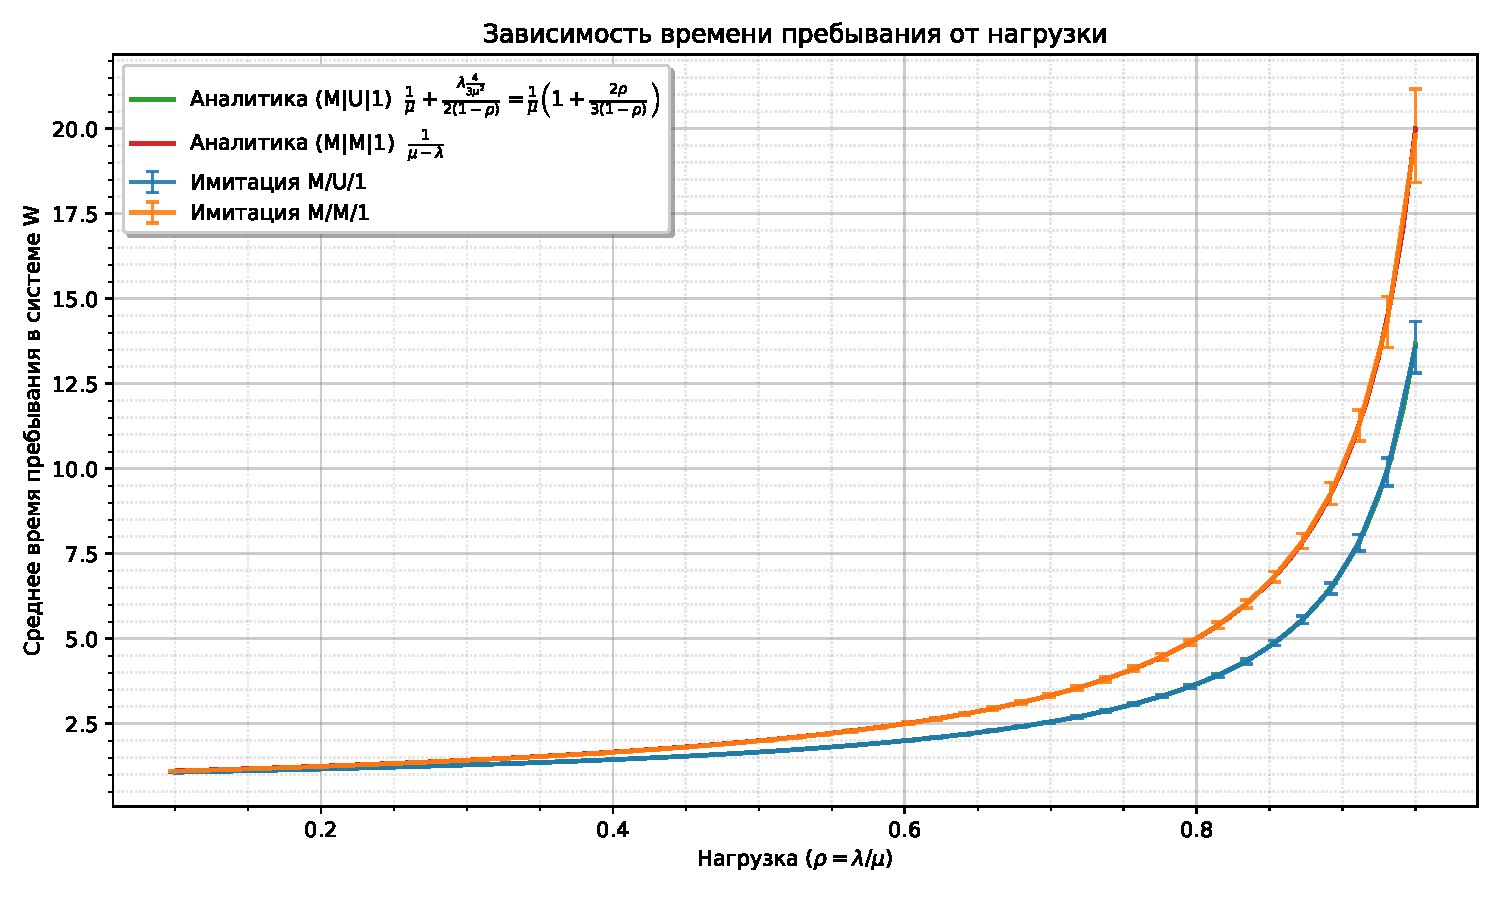
\includegraphics[width=1\textwidth]{mu1.pdf}
    \caption{Сравнение времени пребывания от нагрузки для M/U/1 и M/M/1}
\end{figure}

\section*{3. Исследование M/M/c/c (система с отказами)}
Это многоканальная система, в которой отсутствует очередь: если все $c$ каналов заняты, поступающая заявка отбрасывается (теряется). 

Вероятность отказа (блокировки) вычисляется по первой формуле Эрланга (Erlang B):
\[ P_B = \frac{\frac{\rho^c}{c!}}{\sum_{k=0}^{c} \frac{\rho^k}{k!}} \]

Среднее время пребывания в такой системе для \textit{принятых} заявок не зависит от нагрузки и количества каналов:
\[ W = E[S] = \frac{1}{\mu} \]

\begin{figure}[H]
    \centering
    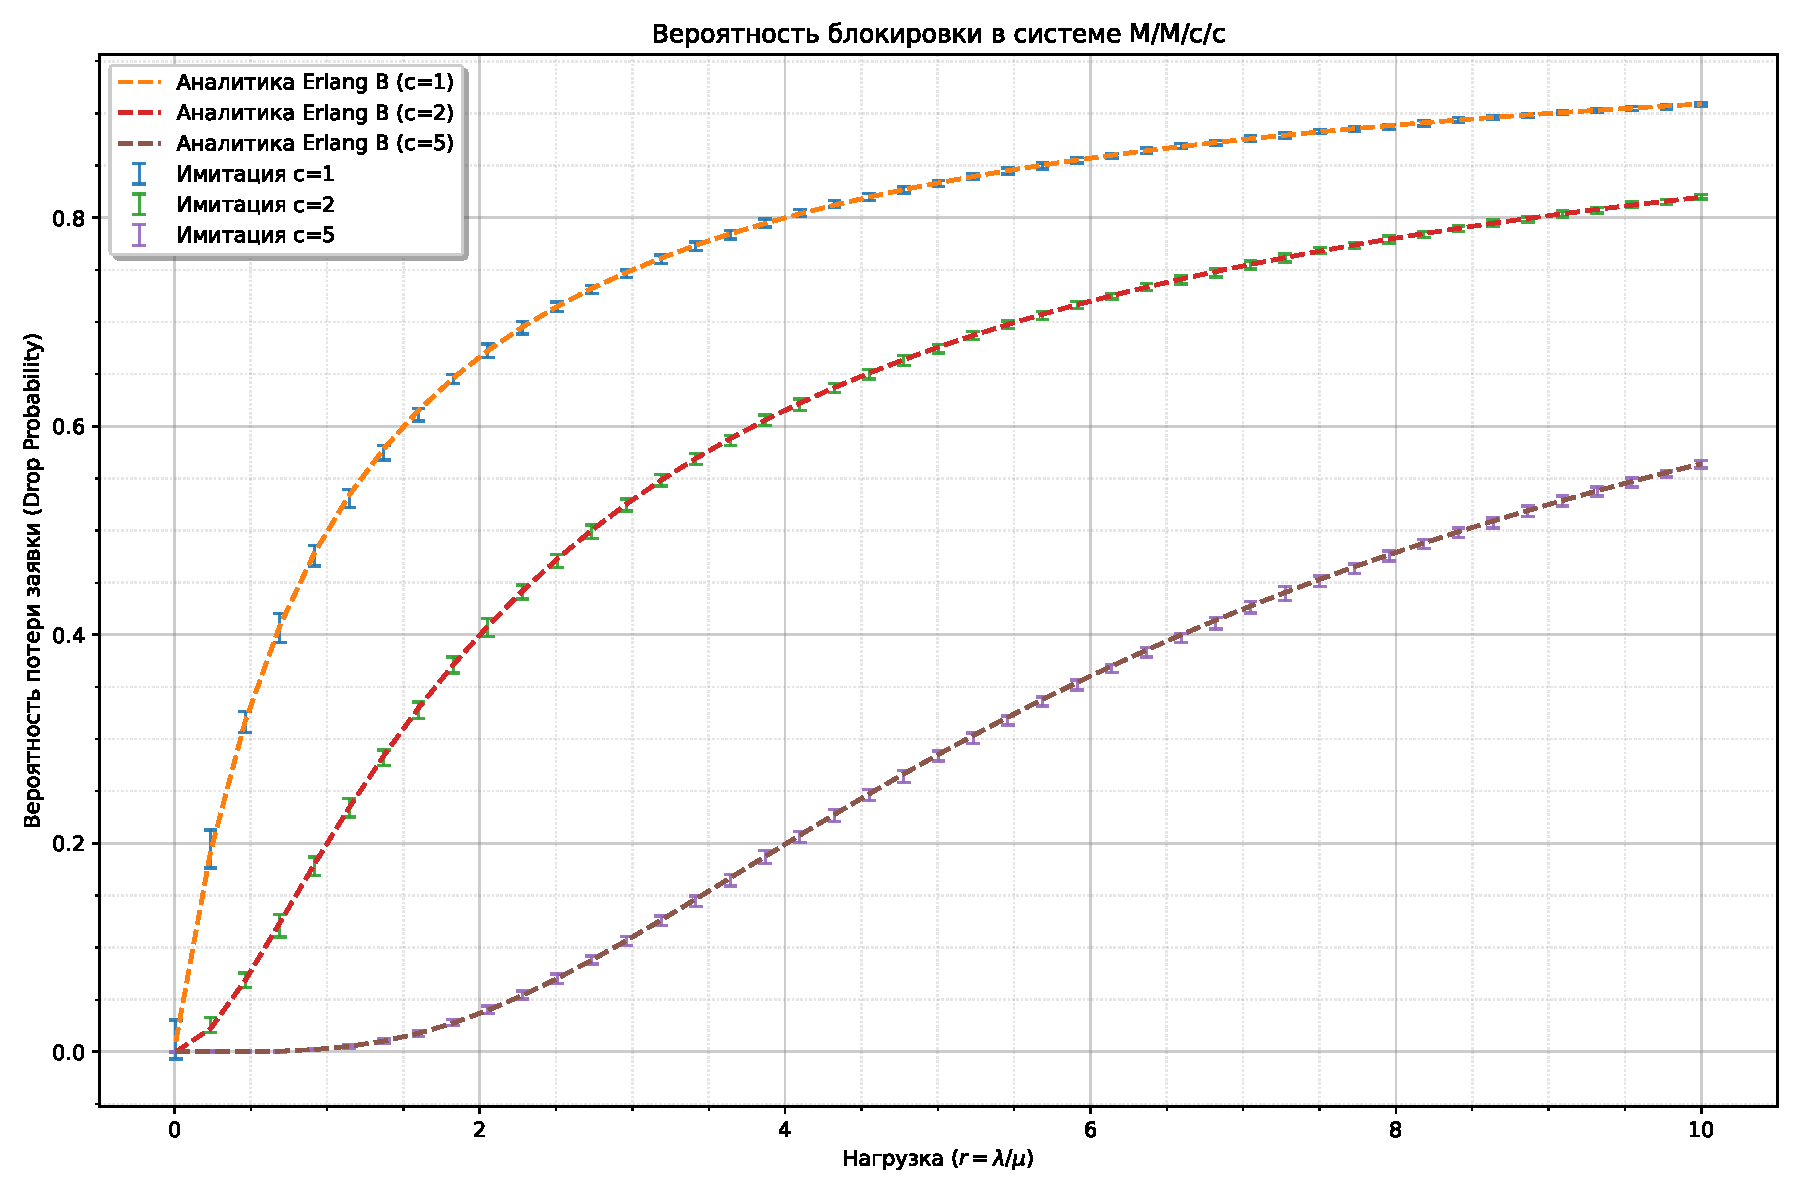
\includegraphics[width=1\textwidth]{mmcc_drop.pdf}
    \caption{Вероятность блокировки заявок в системе M/M/c/c}
\end{figure}

\begin{figure}[H]
    \centering
    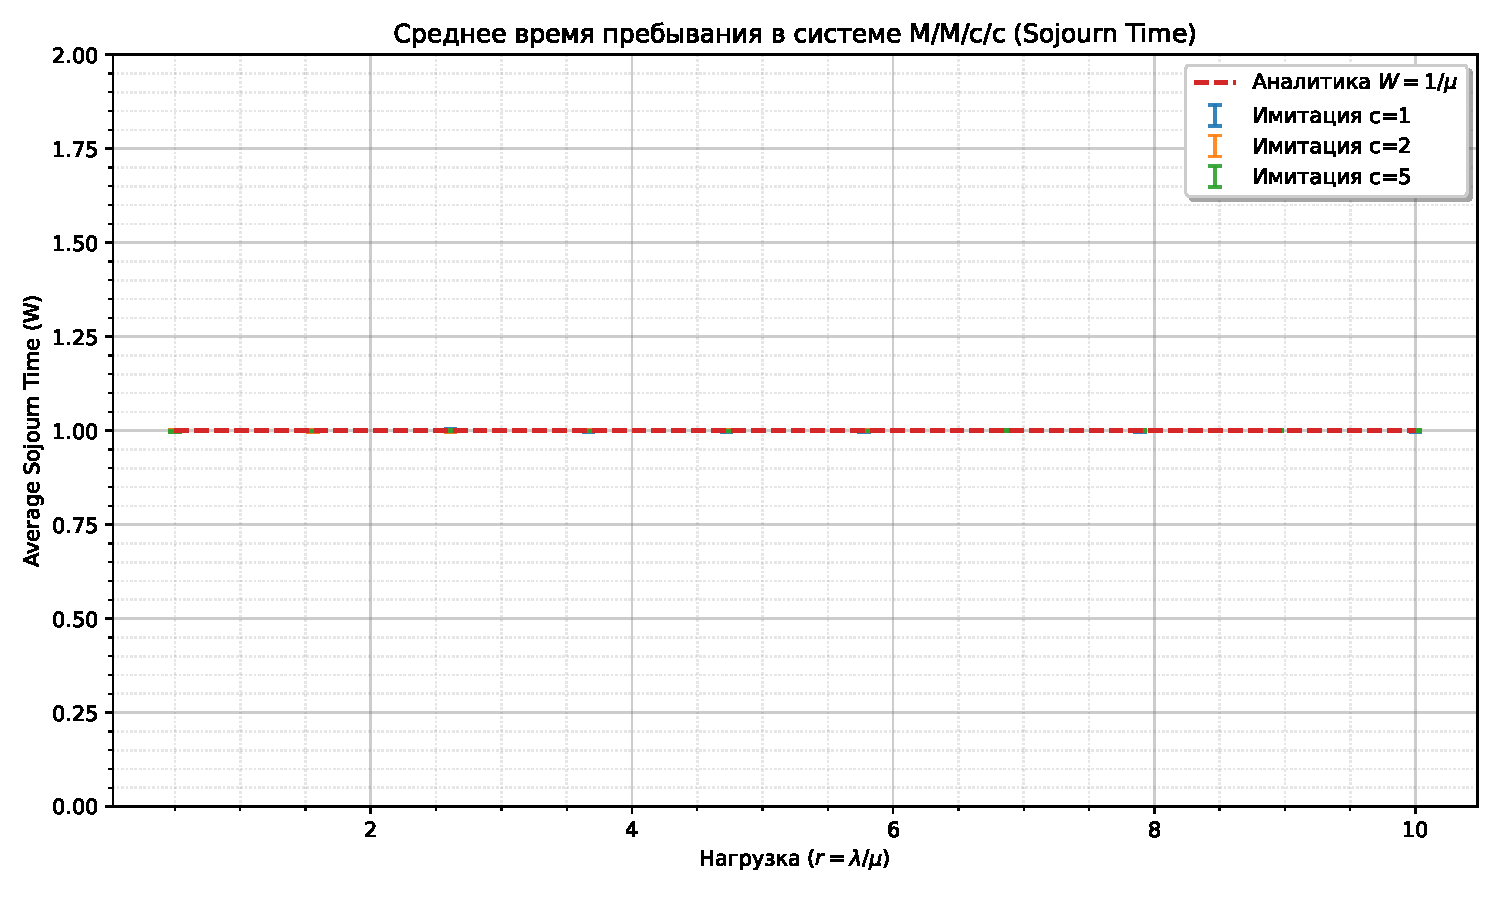
\includegraphics[width=1\textwidth]{mmcc_time.pdf}
    \caption{Среднее время пребывания заявок в системе M/M/c/c}
\end{figure}

\section*{Выводы}
\begin{enumerate}
    \item \textbf{M/M/1:} Имитационная модель работает корректно, эмпирические данные полностью совпадают с аналитической кривой.
    \item \textbf{M/U/1:} Подтверждено, что для равномерного распределения дисперсия меньше, чем для экспоненциального. Как следствие, очередь и общее время нахождения в системе растут медленнее. 
    \item \textbf{M/M/c/c:} Показано, что среднее время пребывания успешно обслуженной заявки в системе без буфера равно времени обслуживания и не зависит от числа серверов. При увеличении числа серверов система способна выдерживать б\'{о}льшие нагрузки при одинаковом уровне потерь.
\end{enumerate}

\end{document}